\documentclass[tikz,border=2pt]{standalone}
\usepackage{amsmath,amssymb}
\usepackage{pgfplots}
\pgfplotsset{compat=1.18}
\usetikzlibrary{arrows.meta}
\begin{document}
% M/M/infinity self-service shop: lambda = 12 per hour, E[S] = 10 minutes, lambda/mu = 2;
% L ~ Pois(2): p(n) = e^{-2} 2^n/n! for n = 0..8; mean E[L] = 2.
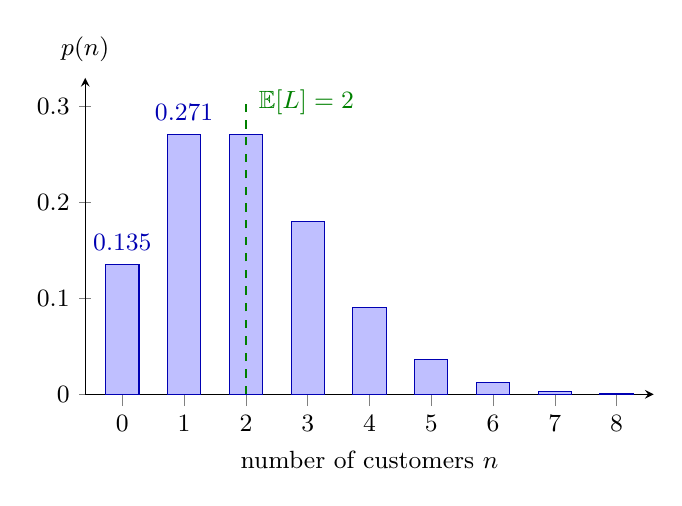
\begin{tikzpicture}[font=\small, >={Latex[length=2mm]}]
  \begin{axis}[
    axis lines=left, xmin=-0.6, xmax=8.6, ymin=0, ymax=0.33,
    xtick={0,...,8}, ytick={0,0.1,0.2,0.3},
    yticklabel style={/pgf/number format/fixed, /pgf/number format/precision=1},
    ybar, bar width=12pt, bar shift=0pt,
    xlabel={number of customers $n$}, ylabel={$p(n)$},
    ylabel style={rotate=-90, anchor=south, at={(axis description cs:0,1.02)}},
    width=8.8cm, height=5.6cm, clip=false]
    \addplot[draw=blue!70!black, fill=blue!25] coordinates {(0,0.1353) (1,0.2707) (2,0.2707) (3,0.1804) (4,0.0902) (5,0.0361) (6,0.0120) (7,0.0034) (8,0.0009)};
    \draw[green!50!black, thick, dashed] (axis cs:2,0) -- (axis cs:2,0.31);
    \node[green!50!black, anchor=west] at (axis cs:2.05,0.305) {$\mathbb{E}[L]=2$};
    \node[blue!70!black, anchor=south] at (axis cs:0,0.14) {$0.135$};
    \node[blue!70!black, anchor=south] at (axis cs:1,0.275) {$0.271$};
  \end{axis}
\end{tikzpicture}
\end{document}
